\section{Conclusão}
\label{sec:conclusao}
Com uma determinada padronização do modelo de branching e versionamento de projetos, é tendência diminuir a ocorrência dos problemas do inferno de dependências (dependency hell) do projeto. No atual presente da escrita deste artigo, tal modelo ainda não foi testado, não sendo possível comprovar a sua eficácia. Uma visão geral do modelo pode ser visto na figura \ref{fig:branching}.

\begin{figure}[h!]
	\centering
	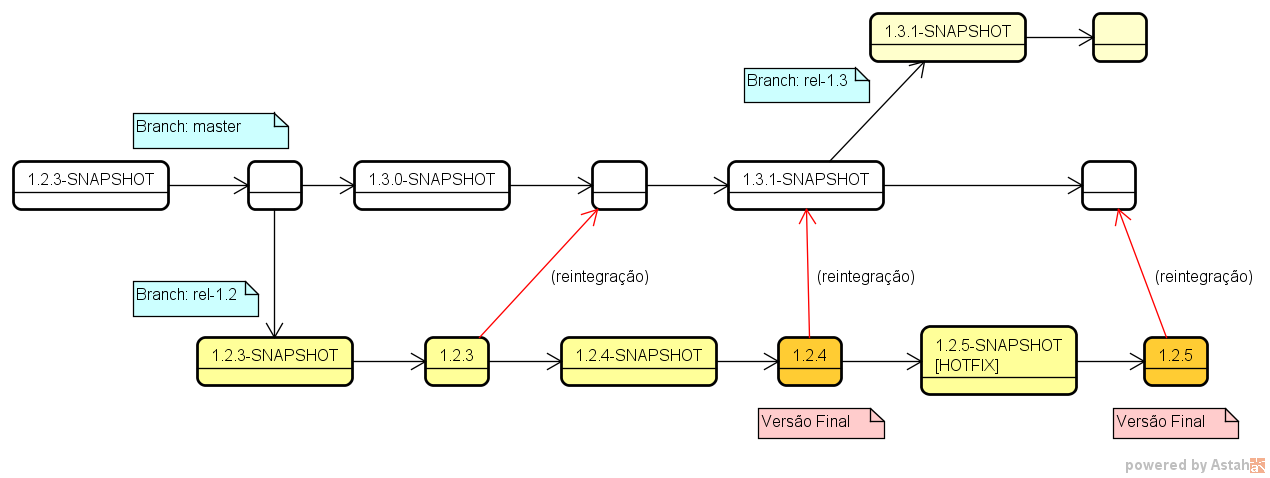
\includegraphics[width=1\linewidth]{img/branching_otojr}
	\caption[Modelo de branching]{Modelo de branching porposto}
	\label{fig:branching}
\end{figure}